\documentclass[a4paper, 12pt]{article}
\usepackage[T2A]{fontenc}
\usepackage[utf8]{inputenc}
\usepackage[english,russian]{babel}
\usepackage{titletoc}
\usepackage{graphicx}
\usepackage{array}
\usepackage{etoolbox}
\usepackage{subfig}
\newcolumntype{P}[1]{>{\centering\arraybackslash}p{#1}}
\def\textunderset#1#2{\leavevmode
  \vtop{\offinterlineskip\halign{%
    \hfil##\hfil\cr\strut#2\cr\noalign{\kern-.3ex}
    \hidewidth\strut#1\hidewidth\cr}}}
\def\signhrule{\raggedright\baselineskip30.0ex \vrule height 0.5pt width30mm depth0pt}


\dottedcontents{section}[2.5em]{\bfseries}{2em}{0.5pc}
\dottedcontents{subsection}[3em]{}{2em}{0.5pc}

\usepackage{hyperref}
\hypersetup{
    colorlinks=true, %set true if you want colored links
    linktoc=all,     %set to all if you want both sections and subsections linked
    linkcolor=black,  %choose some color if you want links to stand out
}

\usepackage{verbatim}

\usepackage{listings}
\usepackage{xcolor}

\lstset
{%
	extendedchars=\true,
	inputencoding=utf8x,
	keepspaces=true,
	frame=tb,
	escapechar=|,
	xleftmargin=0.5cm,
	xrightmargin=0.5cm,
	columns=fullflexible,
	numbers=left,
	numbersep=4pt,
	showspaces=false,
	showstringspaces=false,
	breakatwhitespace=true,
	breaklines=true,
	basicstyle=\color{black}\small\sffamily,
	commentstyle=\color{gray}\itshape,
	stringstyle=\color{orange},
	numberstyle=\footnotesize\color{gray},
	keywordstyle=\color{blue}\bfseries,
	emphstyle={\color{blue}\bfseries},
	tabsize=2,
	texcl=true,
}

\lstdefinestyle{text}{
basicstyle=\small\ttfamily,
columns=flexible,
breaklines=true,
breakatwhitespace=true,
literate={\-}{{-\allowbreak}}1,
numbers=none,
postbreak=\mbox{\textcolor{red}{$\hookrightarrow$}\space},
}

\lstloadlanguages{SQL}

\newcommand{\Title}{Отчет о выполнении лабораторной работы}
\newcommand{\TaskType}{лабораторная работа}
\newcommand{\SubTitle}{по дисциплине <<Поддержка принятия решений в системах мониторинга>>}
\newcommand{\LabTitle}{Выявление логических закономерностей по данным мониторинга} 
\newcommand{\Faculty}{<<Информатика и системы управления>>}
\newcommand{\Department}{<<Компьютерные системы и сети (ИУ-6)>>}
\newcommand{\AuthorFull}{Козлов Владимир Михайлович}
\newcommand{\Author}{Козлов В.М.}
\newcommand{\Teacher}{}
\newcommand{\group}{ИУ6-13М}
\newcommand{\Year}{2024}
\newcommand{\Country}{Россия}
\newcommand{\City}{Москва}

\newcommand{\UpperFullOrganisationName}{Министерство науки и высшего образования Российской Федерации}
\newcommand{\ShortOrganisationName}{МГТУ~им.~Н.Э.~Баумана}
\newcommand{\FullOrganisationName}{федеральное государственное бюджетное образовательное учреждение высшего профессионального образования\newline <<Московский государственный технический университет имени Н.Э.~Баумана (национальный исследовательский университет)>> (\ShortOrganisationName)}

\textwidth=163mm
\textheight=220mm
\oddsidemargin=-0.5pt
\footskip=30pt
\topmargin=27pt
\headheight=12pt
\headsep=25pt
\topskip=10pt
\baselineskip=15pt
\topmargin=-4mm
\begin{document}
\vspace*{-\baselineskip}
\vspace*{-\headheight}
\vspace*{-\headsep}
\vspace*{-2pt}
\thispagestyle{empty}
\begin{center}

% Шапка
{\centering
\begin{tabular}{P{0.15\textwidth}P{0.85\textwidth}}
\smash{
		\raisebox{-0.9\height}{
		
\includegraphics[width=0.15\textwidth]{includes/bmstu.pdf}
		}}
 & \UpperFullOrganisationName\newline \FullOrganisationName \\
\hline
\multicolumn{1}{p{0.15\textwidth}}{} & \multicolumn{1}{p{0.85\textwidth}}{} \\
\multicolumn{1}{p{0.15\textwidth}}{ФАКУЛЬТЕТ}	&	\multicolumn{1}{p{0.85\textwidth}}{\Faculty}	\\
\multicolumn{1}{p{0.15\textwidth}}{КАФЕДРА}	&	\multicolumn{1}{p{0.85\textwidth}}{\Department}	\\
\end{tabular}}
\vfil

{% Основная часть
\vfil
\Large
\underline{\MakeUppercase{\Title}}
\newline
\SubTitle
\vfil
\large
\begin{tabular}{p{0.3\textwidth}p{0.5\textwidth}} 
	Студент:	& \AuthorFull \\ 
	\hline
	Группа:	& \group \\ 
	\hline
	Тип задания:	& \TaskType \\ 
	\hline
	Тема:	& \LabTitle \\ 
	\hline
	\end{tabular}

\vfil

\begin{tabular}{p{0.45\textwidth}p{0.25\textwidth}P{0.25\textwidth}} 
\large
Студент	&	\textunderset{\scriptsize{подпись, дата}}{\signhrule} & \textunderset{\scriptsize{Фамилия, И.О.}}{\ifdefempty{\Author}{\signhrule}{\underline{\Author}}} \\ 
& & \\
Преподаватель	&	\textunderset{\scriptsize{подпись, дата}}{\signhrule} & \textunderset{\scriptsize{Фамилия, И.О.}}{\ifdefempty{\Teacher}{\signhrule}{\underline{\Teacher}}} \\ 
\end{tabular}
}

\vfil
\vfil
\City, \Year

\end{center}

\pagebreak
\tableofcontents
\newpage
% Основная часть --------------------------------------------------------------------------------------------
\section*{Цель}
\addcontentsline{toc}{section}{Цель}
исследовать информационный процесс в системе мониторинга с
помощью методологии IDEF0.
\section*{Задание}
\addcontentsline{toc}{section}{Задание}
С помощью методологии IDEF0 смоделировать диаграммы
“как есть” и “как должно быть” для исследуемого информационного процесса.
\section*{Выбранный процесс}
Процессом для моделирования был выбран процесс разработки плана лечения больного в больнице.
\newpage
% -------------------------------------------------------
\section{Как есть (AS-IS)}
На вход, очевидно, будет подаваться сам больной. \\
Столь же очевидно, что на выходе мы должны получать план лечения.\\
Управляющими данными выступают медицинские пособия с указаниями по лечению и ресурсы, которыми располагает больница, а также амбулаторная карта пациента. \\
"Механизмами" в данном случае выступают врачи и младший медицинский персонал.
\begin{center}
  \centering
  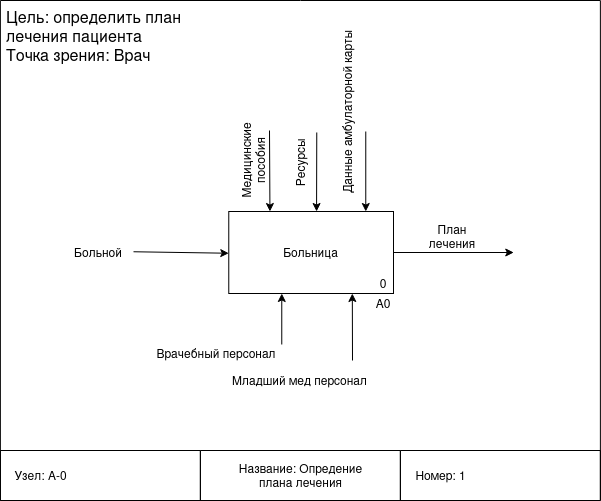
\includegraphics[width=1\linewidth]{extra/as-is_context.png}
  \captionof{figure}{Контекстная диаграмма as-is, A-0}
  \label{fig:prplot}
\end{center}
\subsection{Декомпозиция}
Рассмотрим модели дальнейшей декомпозиции.
\subsubsection{A0}
\begin{center}
  \centering
  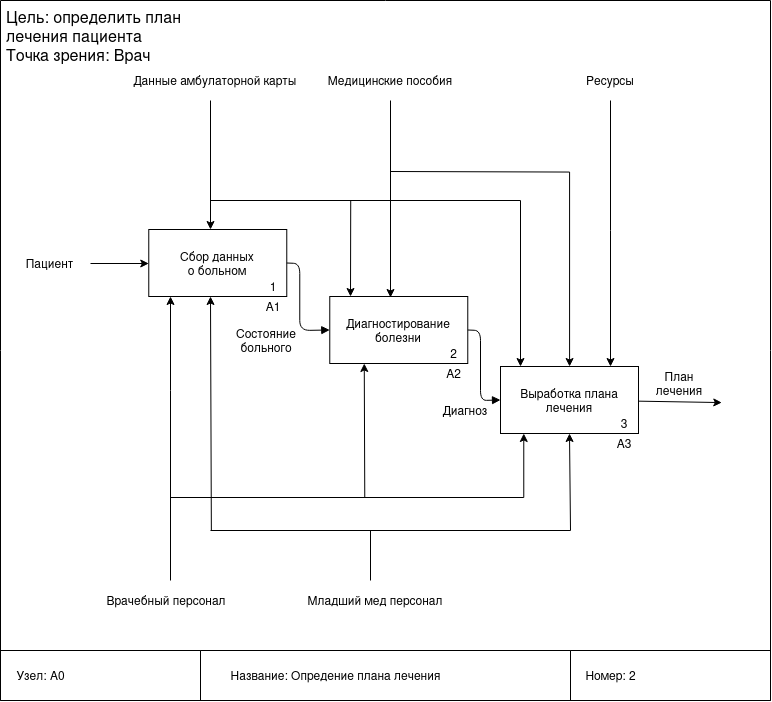
\includegraphics[width=1\linewidth]{extra/as-is_A0.png}
  \captionof{figure}{Декомпозиция блока A0, as-is}
  \label{fig:prplot}
\end{center}
Уровень А0 делится на 3 уровня:
\begin{enumerate}
  \item Сбор данных. Врачи и медсётсры должны как можно больше узнать о состоянии пациента.
  \item Диагностирование болезни. Врачи должны выяснить чем болен пациент.
  \item Выработка плана лечения. Врачи должны выработать план лечения исходя из возможностей (ресурсов) больницы. О ресурсах больше всего осведомлён младший медицинский персонал.
\end{enumerate}
%-----------------
\subsubsection{A1}
\begin{center}
  \centering
  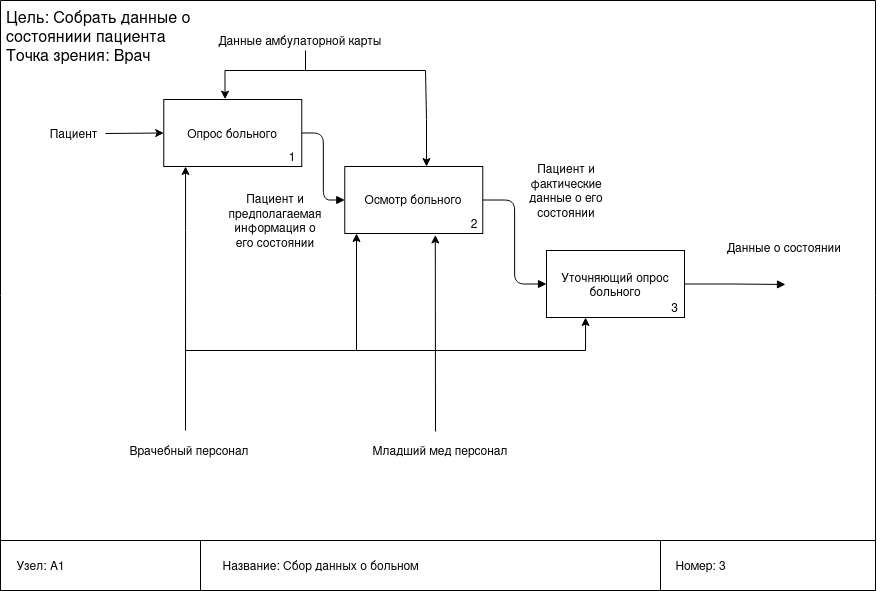
\includegraphics[width=1\linewidth]{extra/as-is_A1.png}
  \captionof{figure}{Декомпозиция блока A1, as-is}
  \label{fig:prplot}
\end{center}
Уровень А1 делится на 3 уровня:
\begin{enumerate}
  \item Опрос больного. Медработникам нужно узнать от пациента зацепки для будущего диагноза и осмотра критических мест.
  \item Осмотр больного. Медработникам нужно осмотреть пациента для получения достоверной информации о его состоянии.
  \item Уточняющий опрос. Медработникам нужно уточнить у пациента данные, полученные при осмотре.
\end{enumerate}
%-----------------
\subsubsection{A2}
\begin{center}
  \centering
  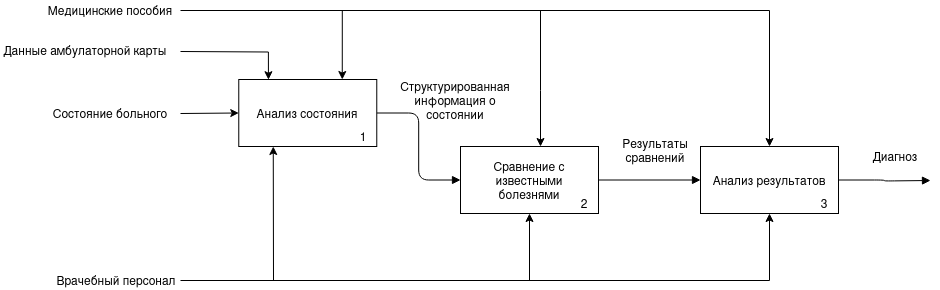
\includegraphics[width=1\linewidth]{extra/as-is_A2.png}
  \captionof{figure}{Декомпозиция блока A2, as-is}
  \label{fig:prplot}
\end{center}
Уровень А2 делится на 3 уровня:
\begin{enumerate}
  \item Анализ состояния. Из набора данных о пациенте нужно получить систему знаний о его состоянии.
  \item Сравнение с известными болезнями. Для выяснения вариантов диагноза нужно сначала выделить вероятные варианты.
  \item Анализ результатов. Исходя из вариантов диагноза нужно выбрать наиболее вероятный.
\end{enumerate}
%-----------------
\subsubsection{A3}
\begin{center}
  \centering
  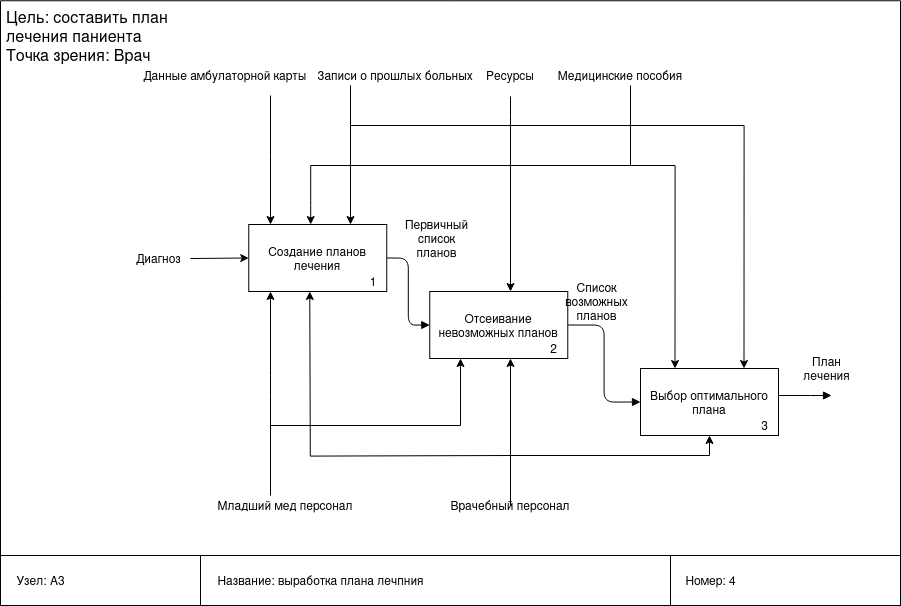
\includegraphics[width=1\linewidth]{extra/as-is_A3.png}
  \captionof{figure}{Декомпозиция блока A3, as-is}
  \label{fig:prplot}
\end{center}
Уровень А3 делится на 3 уровня:
\begin{enumerate}
  \item Создание планов решения. Врачам требуется создать набор планов лечения диагностированной болезни.
  \item Отсеивание невозможных планов. Часть планов нереализуема в этой больнице, а значит должна быть отметена.
  \item Выбор оптимального плана. Из возможных планов нужно выбрать оптимальный.
\end{enumerate}
% -------------------------------------------------------
\section{Как должно быть (TO-BE)}
Для улучшения точности диагностирования стоит добавить постоянное использование опыта с прошлыми пациентами. Так как человек не способен в разумные сроки проанализировать всех прошлых пациентов предлагается использовать специализированную систему для этого, например, на основе графовой базы данных.\\
Таким образом в системе появляется новые управляющие данные - записи о прошлых больных и новый механизм - система сравнения пациентов.
\begin{center}
  \centering
  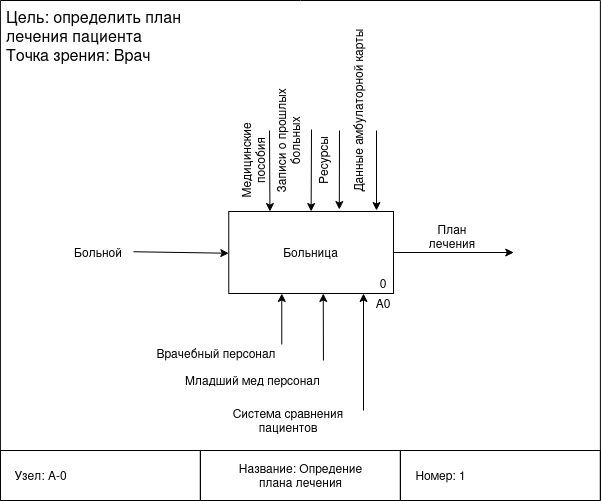
\includegraphics[width=1\linewidth]{extra/to-be_context.png}
  \captionof{figure}{Контекстная диаграмма to-be, A-0}
  \label{fig:prplot}
\end{center}
%-----------------
\subsection{Декомпозиция}
\subsubsection{A0}
\begin{center}
  \centering
  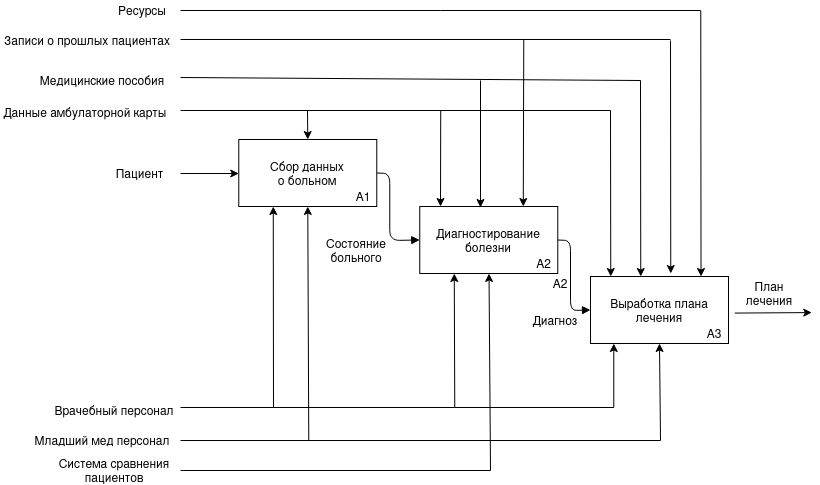
\includegraphics[width=1\linewidth]{extra/to-be_A0.png}
  \captionof{figure}{Декомпозиция блока A0, to-be}
  \label{fig:prplot}
\end{center}
На уровне A0 добавились введённые выше управляюшие данные и механизм, они все воздействуют на уровень A2.
%-----------------
\subsubsection{A2}
\begin{center}
  \centering
  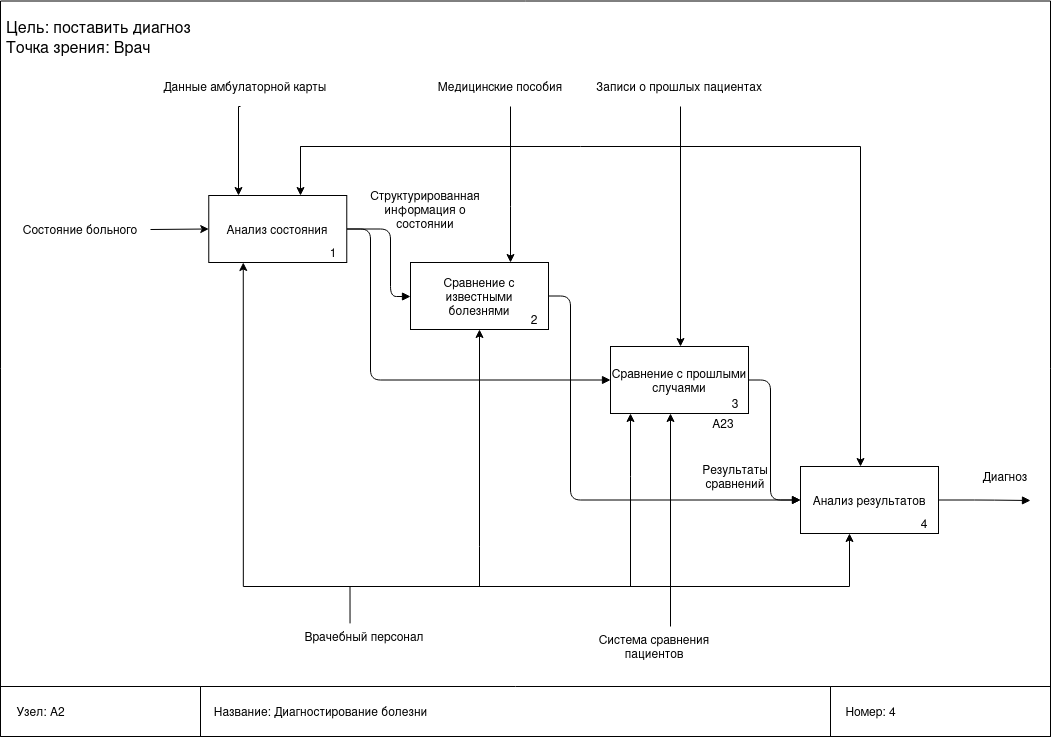
\includegraphics[width=1\linewidth]{extra/to-be_A2.png}
  \captionof{figure}{Декомпозиция блока A2, to-be}
  \label{fig:prplot}
\end{center}
На уровне A2 добавились введённые выше управляюшие данные и механизм, а также новый блок сравнения с прошлыми случаями, который встал параллельно с блоком сравнения с известными болезнями.
%-----------------
\subsubsection{A23}
\begin{center}
  \centering
  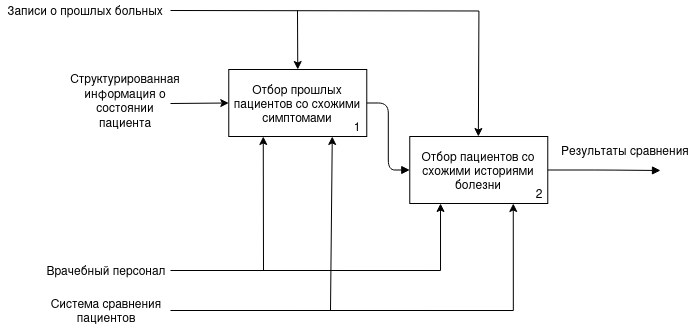
\includegraphics[width=1\linewidth]{extra/to-be_A23.png}
  \captionof{figure}{Декомпозиция блока A23, to-be}
  \label{fig:prplot}
\end{center}
Уровень А23 делится на 3 уровня:
\begin{enumerate}
  \item Отбор прошлых пациентв со схожими симптомами. Так как нет смысла сравнивать нынешнего пациента с не имеющими с ним ничего общего случаями, они отсеиваются.
  \item Отбор пациентов со схожими историями болезни. Для большей схожести следует отобрать случаи, которые ещё и по истории болезни схожи с данным пациентом.
  \item Анализ остальных обстоятельств. Требуется принять во внимание аллергии и прочие обстоятельства при сравнении пациентов.
\end{enumerate}
\newpage
%---------------------------------------------------------
\section{Вывод}
При выполнении домашней работы с помощью
методологии IDEF0 была исследован и улучшен информационный процесс.
\end{document}
